\definecolor{orangecustom}{RGB}{230,115,0}
\definecolor{bluecustom}{RGB}{0,51,102}

\begin{figure}[t]
    \centering
    \includegraphics[width=1\textwidth]{LOGOS/Screenshot 2024-08-22 214355.png}
\end{figure}

\vspace{1.5cm}

\begin{center}
 {\Large\bfseries\textbf{DÉPARTEMENT MATHÉMATIQUES ET INFORMATIQUE}}

    \vspace{1cm}

    {\large\bfseries Filière :}\\
    \vspace{0.5cm}
     {\color{bluecustom}\large\bfseries «Ingénierie Informatique: Big Data et Cloud Computing»}

{\color{bluecustom}\large\bfseries «Génie du Logiciel et des Systèmes Informatiques Distribués»}
{\color{bluecustom}\large\bfseries «Ingénierie Informatique - Cybersécurité et Confiance Numérique»}

    \vspace{0.6cm}

    {\color{black}\Huge\bfseries\textbf{Rapport du\\[0.2cm] Projet d'innovation}}
    \vspace{1cm}

    
\begin{tikzpicture}
        % Define the rectangle with the text
        \node[draw=orangecustom, rectangle, line width=2pt, inner sep=20pt, text width=0.7\textwidth, align=center] (box) {
            \color{black}\Huge{Projet d'innovation : Job-Ai  }
        };

        % Draw two lines inside the rectangle
        \draw[orangecustom, thick] (box.south west) -- (box.south east); % Bottom line
        \draw[orangecustom, thick] (box.north west) -- (box.north east); % Top line
    \end{tikzpicture}

    \vspace{1.4cm}

    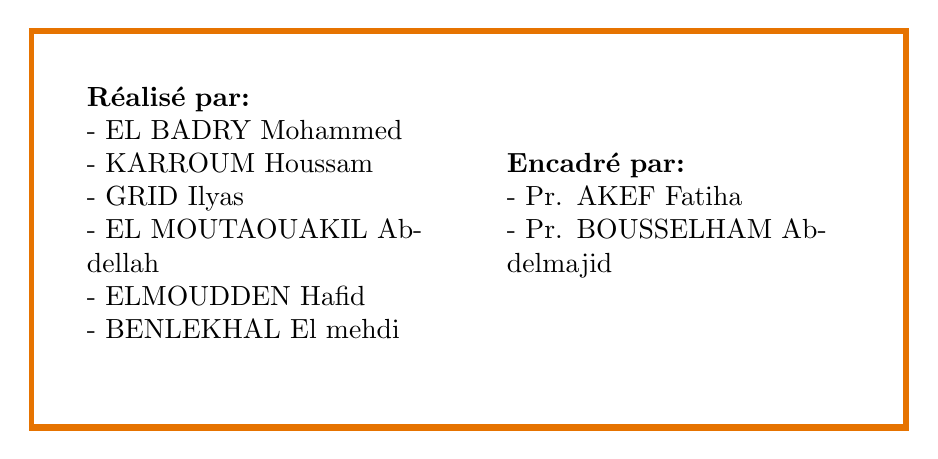
\begin{tikzpicture}
        % Define the rectangle with the text
        \node[draw=orangecustom, rectangle, line width=2pt, inner sep=20pt, text width=0.8\textwidth, align=center] (box) {
            \begin{minipage}{0.45\textwidth}
                \textbf{Réalisé par:}\\
                    - EL BADRY Mohammed\\
                    - KARROUM Houssam\\
                    - GRID Ilyas\\
                    - EL MOUTAOUAKIL Abdellah\\
                    - ELMOUDDEN Hafid\\
                    - BENLEKHAL El mehdi\\
            \end{minipage}
            \hfill
            \begin{minipage}{0.45\textwidth}
                \textbf{Encadré par:}\\
                       - Pr. AKEF Fatiha\\
                       - Pr. BOUSSELHAM Abdelmajid\\
            \end{minipage}
        };

        % Draw two lines inside the rectangle
        \draw[orangecustom, thick] (box.south west) -- (box.south east); % Bottom line
        \draw[orangecustom, thick] (box.north west) -- (box.north east); % Top line
    \end{tikzpicture}

    \vfill

    {\large\bfseries Année Universitaire: 2024-2025}
\end{center}

\vfill

% Footer
\begin{figure}[b]
    \centering
    \includegraphics[width=1\textwidth]{LOGOS/Screenshot 2024-08-22 214411.png}
\end{figure}